% Options for packages loaded elsewhere
% Options for packages loaded elsewhere
\PassOptionsToPackage{unicode,linktoc=all}{hyperref}
\PassOptionsToPackage{hyphens}{url}
\PassOptionsToPackage{dvipsnames,svgnames,x11names}{xcolor}
%
\documentclass[
  ngerman,
  11pt,
  a4paper,
  DIV=11,
  twoside]{scrreprt}
\usepackage{xcolor}
\usepackage[inner=3cm,outer=4cm,top=3cm,bottom=4cm,headsep=22pt,headheight=11pt,footskip=33pt,ignorehead,ignorefoot,heightrounded]{geometry}
\usepackage{amsmath,amssymb}
\setcounter{secnumdepth}{2}
\usepackage{iftex}
\ifPDFTeX
  \usepackage[T1]{fontenc}
  \usepackage[utf8]{inputenc}
  \usepackage{textcomp} % provide euro and other symbols
\else % if luatex or xetex
  \usepackage{unicode-math} % this also loads fontspec
  \defaultfontfeatures{Scale=MatchLowercase}
  \defaultfontfeatures[\rmfamily]{Ligatures=TeX,Scale=1}
\fi
\usepackage{lmodern}
\ifPDFTeX\else
  % xetex/luatex font selection
  \setmainfont[]{Calibri}
  \setmathfont[]{TeX Gyre Termes Math}
\fi
% Use upquote if available, for straight quotes in verbatim environments
\IfFileExists{upquote.sty}{\usepackage{upquote}}{}
\IfFileExists{microtype.sty}{% use microtype if available
  \usepackage[]{microtype}
  \UseMicrotypeSet[protrusion]{basicmath} % disable protrusion for tt fonts
}{}
\makeatletter
\@ifundefined{KOMAClassName}{% if non-KOMA class
  \IfFileExists{parskip.sty}{%
    \usepackage{parskip}
  }{% else
    \setlength{\parindent}{0pt}
    \setlength{\parskip}{6pt plus 2pt minus 1pt}}
}{% if KOMA class
  \KOMAoptions{parskip=half}}
\makeatother
% Make \paragraph and \subparagraph free-standing
\makeatletter
\ifx\paragraph\undefined\else
  \let\oldparagraph\paragraph
  \renewcommand{\paragraph}{
    \@ifstar
      \xxxParagraphStar
      \xxxParagraphNoStar
  }
  \newcommand{\xxxParagraphStar}[1]{\oldparagraph*{#1}\mbox{}}
  \newcommand{\xxxParagraphNoStar}[1]{\oldparagraph{#1}\mbox{}}
\fi
\ifx\subparagraph\undefined\else
  \let\oldsubparagraph\subparagraph
  \renewcommand{\subparagraph}{
    \@ifstar
      \xxxSubParagraphStar
      \xxxSubParagraphNoStar
  }
  \newcommand{\xxxSubParagraphStar}[1]{\oldsubparagraph*{#1}\mbox{}}
  \newcommand{\xxxSubParagraphNoStar}[1]{\oldsubparagraph{#1}\mbox{}}
\fi
\makeatother


\usepackage{longtable,booktabs,array}
\newcounter{none} % for unnumbered tables
\usepackage{calc} % for calculating minipage widths
% Correct order of tables after \paragraph or \subparagraph
\usepackage{etoolbox}
\makeatletter
\patchcmd\longtable{\par}{\if@noskipsec\mbox{}\fi\par}{}{}
\makeatother
% Allow footnotes in longtable head/foot
\IfFileExists{footnotehyper.sty}{\usepackage{footnotehyper}}{\usepackage{footnote}}
\makesavenoteenv{longtable}
\usepackage{graphicx}
\makeatletter
\newsavebox\pandoc@box
\newcommand*\pandocbounded[1]{% scales image to fit in text height/width
  \sbox\pandoc@box{#1}%
  \Gscale@div\@tempa{\textheight}{\dimexpr\ht\pandoc@box+\dp\pandoc@box\relax}%
  \Gscale@div\@tempb{\linewidth}{\wd\pandoc@box}%
  \ifdim\@tempb\p@<\@tempa\p@\let\@tempa\@tempb\fi% select the smaller of both
  \ifdim\@tempa\p@<\p@\scalebox{\@tempa}{\usebox\pandoc@box}%
  \else\usebox{\pandoc@box}%
  \fi%
}
% Set default figure placement to htbp
\def\fps@figure{htbp}
\makeatother


% definitions for citeproc citations
\NewDocumentCommand\citeproctext{}{}
\NewDocumentCommand\citeproc{mm}{%
  \begingroup\def\citeproctext{#2}\cite{#1}\endgroup}
\makeatletter
 % allow citations to break across lines
 \let\@cite@ofmt\@firstofone
 % avoid brackets around text for \cite:
 \def\@biblabel#1{}
 \def\@cite#1#2{{#1\if@tempswa , #2\fi}}
\makeatother
\newlength{\cslhangindent}
\setlength{\cslhangindent}{1.5em}
\newlength{\csllabelwidth}
\setlength{\csllabelwidth}{3em}
\newenvironment{CSLReferences}[2] % #1 hanging-indent, #2 entry-spacing
 {\begin{list}{}{%
  \setlength{\itemindent}{0pt}
  \setlength{\leftmargin}{0pt}
  \setlength{\parsep}{0pt}
  % turn on hanging indent if param 1 is 1
  \ifodd #1
   \setlength{\leftmargin}{\cslhangindent}
   \setlength{\itemindent}{-1\cslhangindent}
  \fi
  % set entry spacing
  \setlength{\itemsep}{#2\baselineskip}}}
 {\end{list}}
\usepackage{calc}
\newcommand{\CSLBlock}[1]{\hfill\break\parbox[t]{\linewidth}{\strut\ignorespaces#1\strut}}
\newcommand{\CSLLeftMargin}[1]{\parbox[t]{\csllabelwidth}{\strut#1\strut}}
\newcommand{\CSLRightInline}[1]{\parbox[t]{\linewidth - \csllabelwidth}{\strut#1\strut}}
\newcommand{\CSLIndent}[1]{\hspace{\cslhangindent}#1}

\ifLuaTeX
\usepackage[bidi=basic,shorthands=off]{babel}
\else
\usepackage[bidi=default,shorthands=off]{babel}
\fi
\ifPDFTeX
\else
\babelfont{rm}[]{Calibri}
\fi
\ifLuaTeX
  \usepackage{selnolig} % disable illegal ligatures
\fi


\setlength{\emergencystretch}{3em} % prevent overfull lines

\providecommand{\tightlist}{%
  \setlength{\itemsep}{0pt}\setlength{\parskip}{0pt}}



 


\usepackage{circuitikz}
\usetikzlibrary{arrows.meta}
\KOMAoption{captions}{tableheading}
\makeatletter
\@ifpackageloaded{caption}{}{\usepackage{caption}}
\AtBeginDocument{%
\ifdefined\contentsname
  \renewcommand*\contentsname{Inhaltsverzeichnis}
\else
  \newcommand\contentsname{Inhaltsverzeichnis}
\fi
\ifdefined\listfigurename
  \renewcommand*\listfigurename{Abbildungsverzeichnis}
\else
  \newcommand\listfigurename{Abbildungsverzeichnis}
\fi
\ifdefined\listtablename
  \renewcommand*\listtablename{Tabellenverzeichnis}
\else
  \newcommand\listtablename{Tabellenverzeichnis}
\fi
\ifdefined\figurename
  \renewcommand*\figurename{Abbildung}
\else
  \newcommand\figurename{Abbildung}
\fi
\ifdefined\tablename
  \renewcommand*\tablename{Tabelle}
\else
  \newcommand\tablename{Tabelle}
\fi
}
\@ifpackageloaded{float}{}{\usepackage{float}}
\floatstyle{ruled}
\@ifundefined{c@chapter}{\newfloat{codelisting}{h}{lop}}{\newfloat{codelisting}{h}{lop}[chapter]}
\floatname{codelisting}{Listing}
\newcommand*\listoflistings{\listof{codelisting}{Listingverzeichnis}}
\makeatother
\makeatletter
\makeatother
\makeatletter
\@ifpackageloaded{caption}{}{\usepackage{caption}}
\@ifpackageloaded{subcaption}{}{\usepackage{subcaption}}
\makeatother
\usepackage{bookmark}
\IfFileExists{xurl.sty}{\usepackage{xurl}}{} % add URL line breaks if available
\urlstyle{same}
\hypersetup{
  pdftitle={VCO Design und Simulation},
  pdfauthor={Mirco Ick; Torben Becker; Tassilo Hertling},
  pdflang={de},
  colorlinks=true,
  linkcolor={blue},
  filecolor={Maroon},
  citecolor={Blue},
  urlcolor={Blue},
  pdfcreator={LaTeX via pandoc}}


\title{VCO Design und Simulation}
\author{Mirco Ick \and Torben Becker \and Tassilo Hertling}
\date{2026-07-02}
\begin{document}
\maketitle

\renewcommand*\contentsname{Inhaltsverzeichnis}
{
\setcounter{tocdepth}{2}
\tableofcontents
}

\chapter{Introduction}\label{introduction}

In diesesm Projekt gilt es einen VCO (Voltage Controlled Oszillator) zu
designen und in Betrieb zu nehmen. Das Design soll bestimmte
Anforderungen erfüllen, damit es in einem Laborversuch als FM-Modulator
genutzt werden kann. In der Vergangenheit wurde im Laborversuch eine VCO
Schaltung mit alten und abgekündigkten Komponenten verwendet. Diese
Schaltung soll nun mit neuen und verfügbaren Komponenten erneuert
werden.

Die VCO Schaltung soll eine FM-Modulation mit einem Trägersignal bei der
Frequenz \(5,5~\text{MHz}\) durchführen und einen Modulationsbereich
zwischen \(5~\text{MHz}\) und \(6~\text{MHz}\) verwenden. Der
Einstellungsbereich soll mit \(1~\text{V}\) pro \(1~\text{MHz}\)
eingestellt werden. Somit kann das zu modulierende Signal einen
Spannungsbereich von \(V_{pp} = 1~\text{V}\) haben. Die Ein- und
Ausgangsimpedanz soll \(50~\Omega\) betragen.

Zudem soll die Schaltung aus Komponenten bestehen, die Studierenden im
4.Semester bereits kennen, damit die Schaltung im Rahmen des
Laborversuchs im Grunde verstanden werden kann. Aus dieser
Rahmenbedingung folgt die Auswahl der spezifischen VCO-Schaltung.

Die Platine soll zudem relativ groß ausgelegt werden und es sollen
möglichst bedrahtete Bauteile verwendet werden. In dem Laborversuch soll
ebenfalls die Kennlinie des FM-Modulators aufgenommen werden. Hierfür
ist ein integrierter einstellbarer Spannungsteiler vorgesehen, der über
einen Drehregler auf der Platine eingestellt werden soll.

Die Schaltung soll ebenfalls Stabil gegenüber Schwankungen in der
Versorgungsspannung und somit in der Ausgangsfrequenz ausgelegt sein.
Anschlüsse für die im Laborversuch verwendeten Geräte wie das
Oszilloskop und dem Spektrumanalysator sollen über SMA- oder
BNC-Anschlüsse geschehen.

\chapter{Technische Spezifikationen
(Kundenanforderungen)}\label{technische-spezifikationen-kundenanforderungen}

\begin{itemize}
\item
  \textbf{Mittenfrequenz (\(f_0\)):} \(5,5~\text{MHz}\)
  (Zwischenfrequenz / ZF) bei einer Steuerspannung von \(0~\text{V}\).
\item
  \textbf{Linearer Modulationsbereich:} \(\pm 0,5~\text{MHz}\)
  (Frequenzhub) bei einer Steuerspannung von \(\pm 0,5~\text{V}\).

  \begin{itemize}
  \tightlist
  \item
    \emph{Arbeitsbereich:} \(5,0~\text{MHz}\) bis \(6,0~\text{MHz}\)
    linear im Spannungsbereich von \(-0,5~\text{V}\) bis
    \(+0,5~\text{V}\).
  \end{itemize}
\item
  \textbf{Frequenzstabilität:} Es darf keine Frequenzverschiebung
  (Drift) durch thermische oder externe Einflüsse auftreten.
\item
  \textbf{Systemimpedanz:} Ein- und Ausgangswiderstand müssen exakt
  \(50~\Omega\) betragen.
\item
  \textbf{Steckverbinder:} Ein- und Ausgänge sind als \textbf{SMA-} oder
  \textbf{BNC-Buchsen} auszuführen.
\item
  \textbf{Schaltungsarchitektur:} Einfacher, leicht zu verstehender und
  nachvollziehbarer Aufbau (diskreter Bauelemente).
\item
  \textbf{Spannungsversorgung:} Integrierte Stabilisierung und Filterung
  der Versorgungsspannung zur Rauschunterdrückung.
\item
  \textbf{Manuelle Steuerung:} Integrierter Spannungsteiler mit einem
  analogen Drehknopf (Potentiometer) zur Frequenzeinstellung.
\item
  \textbf{Platinedesign:} Relativ große, robuste und mechanisch
  unempfindliche Leiterplatte.
\item
  \textbf{Bestückungstechnologie:} Ausschließlich \textbf{stehende,
  bedrahtete Bauteile} für optimale Zugänglichkeit (keine SMD-Bauteile).
\end{itemize}

\chapter{Designverlauf}\label{designverlauf}

\section{Grundlegender VCO}\label{grundlegender-vco}

Zuerst wurde im Design angefangen ein passendes VCO-Modell nach den
Anforderungen auszusuchen. Als Modell haben wurde sich für den LC-VCO
entschieden. Dieser besteht im Grunde aus einer RLC-Schaltung und einer
kreuzgekoppelten Mosfet-Schaltung. Das Design ist somit gut für
Studierende aus dem 4. Semester zu verstehen und kann auch gut mit
bedrahteten Bauteilen aufgebaut werden. Die Grundschaltung ist in
Abbildung~\ref{fig-circuit} zu sehen:

\begin{figure}

\centering{

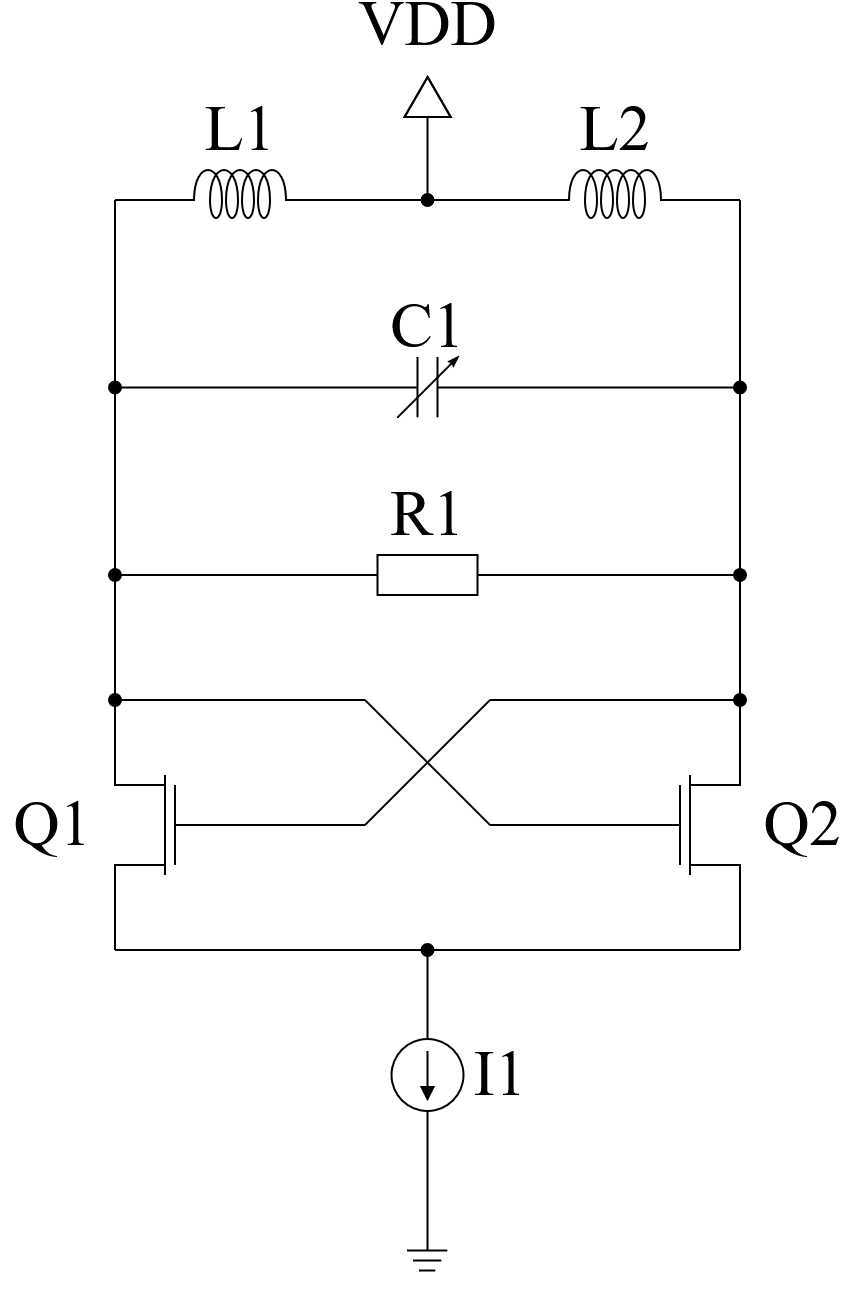
\includegraphics[width=0.6\linewidth,height=\textheight,keepaspectratio]{./images/circuit.png}

}

\caption{\label{fig-circuit}VCO-Grundschaltung}

\end{figure}%

In der Grundschaltung sind im oberen Bereich die beiden Induktivitäten
\(L1\) und \(L2\) in doppelter Ausführung zu sehen, da die
Versorgungsspannung mittig angeschlossen werden muss, um die Symmetrie
der Schaltung gewärleisten zu können. Weiter unten ist der einstellbare
Kondensator \(C1\) zu sehen, dessen Wert die Schwingung der Schaltung
maßgeblich beeinflusst. Durch die Änderung des Kondensator ändert sich
auch die Frequenz \(f_0\) der Schaltung. Somit kann duch eine gesteuerte
Änderung der Kapazität die Frequenz der Schwingung eingestellt werden.
Das ist das Grundprinzip des VCO´s und die Funktionsweise der
FM-Modulation. Der Widerstand \(R1\) vervollständigt den
RLC-Schwingkreis. Die beiden kreugekoppelten Mosfets sind für die
ständige Anregung der Schwingung zuständig. Durch die ständige Änderung
der gesamt Impedanz des Schwingkreises ändert sich jeweils der Strom,
der durch die Mosfets am Gate Eingang anliegt. Diese Änderung bewirkt
eine Rückgekoppelte Schleife, durch welche schwingt das System
dauerhaft. Nach Implementierung dieser Schaltung in KiCad, NG- sowie
LT-Spice konnte die Funktionsweise sowie das Einstellen der Frequenz
\(f_0\) klarer gemacht werden.

Im Verlauf der Entwicklung wurde sich entschieden verschiede VCO Ansätze
zu entwerfen und am Ende dem Kunden zu präsentieren. Unter den drei
Gruppen konnte sich neben dem Grund-VCO, welcher oben bereits erklärt
wurde, der Colpitts Oszillator oder der Wien-Robinson-Oszillator
ausgesucht werden. Da sich bereits im zweiten Semester ausgiebig mit der
Wien-Robinson Brücke auseinander gesetzt wurde haben wir uns für diesen
VCO entschieden, auf welchen in den nachfolgenden Kapiteln näher
eingegangen wird.

Eine Simulationsdatei ist dem Ordner
\href{./kicad/Archiv/VCO-Schwingkreis/}{VCO-Schwingkreis} zu entnehmen.

\section{Wien-Robinson-Oszillator}\label{wien-robinson-oszillator}

Um den Wien-Robinson-Oszillator besser verstehen zu können wurde sich
als erstes die Grundschaltung, die Wien-Robinson-Brücke, nochmals
angeschaut. Hierbei handelt es sich um eine frequenzabhängige
Wechselstrom-Messbrücke, die als sogenannte Nullbrücke konzipiert ist.
Das bedeutet, dass die Differenzspannung in der Brückendiagonale bei
einer spezifischen Resonanzfrequenz exakt
\(\underset{\scriptscriptstyle\sim}{U} = 0~\text{V}\) beträgt. Ein
Schaltung ist der Abbildung~\ref{fig-wienrobbruecke} zu entnehmen.

\begin{figure}

\centering{

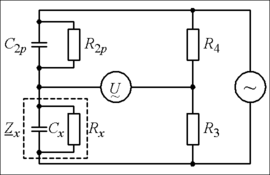
\includegraphics[width=0.7\linewidth,height=\textheight,keepaspectratio]{./images/wien_rob_bruecke.png}

}

\caption{\label{fig-wienrobbruecke}Wien-Robinson-Brücke
({de-academic.com} 2000-2026)}

\end{figure}%

Wenn man nun an diese Brückendiagonale einen Operationsverstärker (OPV)
einbaut, erhält man einen aktiven Oszillator, der die
Frequenzselektivität der Brücke nutzt. Da der OPV die verschwindend
geringe Differenzspannung im Bereich der Resonanzfrequenz extrem hoch
verstärkt, reicht bereits das thermische Rauschen der Bauteile aus, um
das System resonant anzuregen. Somit erhält man einen sich selber
anwingenden Oszillator. Diese Wien-Robinson-Oszillator Schaltung ist
eine der meistgenutzen Schaltungen einer Wien-Robinson-Brücke und bietet
somit eine gute Grundlage des VCO's. Für die ersten Tests mit dem
Wien-Robinson-Oszillator wurde die Seite des Elektroniktutors
herangezogen und versucht, die entsprechende Schaltung nachzustellen
(Mietke 2002-2026).

\begin{figure}

\centering{

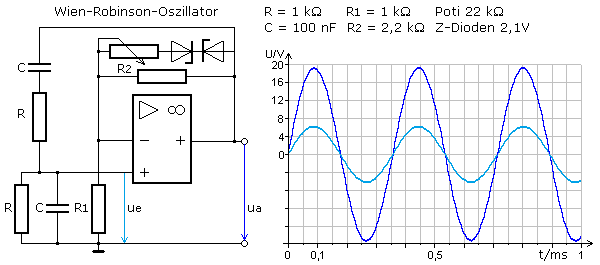
\includegraphics[width=0.8\linewidth,height=\textheight,keepaspectratio]{./images/wien3.png}

}

\caption{\label{fig-wien}Wien-Robinson-Oszillator Schaltung (Mietke
2002-2026)}

\end{figure}%

Die in Abbildung~\ref{fig-wien} zu sehende Schaltung zeigt wie bereits
erörtert den in der Brückendiagonalen eingebaute Operationsverstärker
und eine zusätzliche Amplitudenregulierung. Durch die starke Anregung
der Schwingung des OPV's wurde hier noch eine Amplitudenregelung
eingebaut, welche aus einem Potentiometer und zwei entgegengeschalteten
Varktordioden besteht. Ohne diese Amplitudenregelung würde die
Schwingung aufgrund der unendlichen Verstärkung des OPV schnell bis an
die Grenzen der Versorgungsspannung anwachsen und begrenzen, was zu
starken Verzerrungen des Sinussignals führen würde. Die Regelung sorgt
dafür, dass sich ein stabiler, verzerrungsfreier Dauerschwingzustand
einstellt.

Nachdem nun diese Schaltung erfolgreich in KiCAD, erst auf der
ursprünglichen Resonanzfrequenz \(f_0=1592~\text{Hz}\) und anschließend
mit Änderung des OPV's (LT7171) auf die gewünschten \(5,5~\text{MHz}\),
umgesetzt wurde, konnte sich um den geforderten Frequenzhub von
\(\Delta f=1~\text{MHz}\) bei einer Steuerspannungsänderung von
\(U_{str}=\pm 0,5~\text{V}\) gemacht werden. Für den ersten Entwurf
wurden nun Varaktoren parallel zu den beiden Kondensatoren \(C\)
geschaltet. Ein erster Versuch ist der \textbf{?@fig-wienvarak} zu
entnehemen.

\textbf{Abbildung mit Wien-Robinson-Oszillator mit Frequenzhub}

Nach umsetzen dieser Schaltung haben sich jedoch zwei Probleme
kristallisiert. Zum einen kamen in den verschiedenen Simulationen (KiCAD
bzw. NG-Spice und LT-Spice) unterschiede Ergebnisse heraus, und zum
anderen war es nicht möglich die Kennlinie der Resonanzfrequenz \(f_0\)
über die Steuerspannung \(U_{str}\) linear zu bekommen. Nach vielen
vergeblichen Versuchen wurde sich dann dazu entschieden den kompletten
Aufbau neu aufzusetzen und eine andere Schaltung zu verwenden.

\section{Wien-Robinson VCO}\label{wien-robinson-vco}

\section{Komponenten}\label{komponenten}

Um den Wien-Robinson-Oszilator im gewünschten Berreich zu bekommen
musste die Grundschaltung angepasst werden und entsprechende Bauteile
rausgesucht werden.

\subsection{Operationsverstärker}\label{operationsverstuxe4rker}

Da die Schaltung um \(5~\text{MHz}\) schwingen soll muss der OPV sowohl
ultra-high-speed sein als auch eine hohe Slew-rate haben.

\subsection{Varaktoren}\label{varaktoren}

Damit die Mittenfrequenz verschoben werden kann wurden varaktoren
Parrallel zu den Kondensatoren der Wien-Robinson-Brücke geschaltet. Um
sich in einem Lineraren Berreich zu bewegen müssen die kennlinien der
varaktoren in dem beschalteten Berreich auch linerar sein. Zudem müssen
sie eine Möglichst hohe änderung der Kapazität in diesem Berreich haben.

\subsection{Diode}\label{diode}

?

\subsection{Diode}\label{diode}

\chapter{Charakterisierung}\label{charakterisierung}

\chapter*{Literaturverzeichnis}\label{literaturverzeichnis}
\addcontentsline{toc}{chapter}{Literaturverzeichnis}

\protect\phantomsection\label{refs}
\begin{CSLReferences}{1}{1}
\bibitem[\citeproctext]{ref-wienrobinsonbruecke}
{de-academic.com}. 2000-2026. \emph{Wien-Robinson-Brücke}. Design
Reference. \url{https://de-academic.com/dic.nsf/dewiki/1507065}.

\bibitem[\citeproctext]{ref-wienbruecke}
Mietke, Detlef. 2002-2026. \emph{Wien-Robinson-Oszillator}. Design
Reference.
\url{https://www.elektroniktutor.de/signalkunde/wien_osz.html}.

\end{CSLReferences}




\end{document}
